%% Introduction %%

L'objectif premier, lors de la création d'un outil, est qu'il soit utilisé par le public visé. Il n'y a pas d'intérêt à créer un outil si l'utilisateur ne le trouve pas assez attractif et avantageux pour l'intégrer à ses habitudes. Étant donné que nous souhaitons ajouter cet outil à la grande palette d'outils des utilisateurs des collections, nous avons particulièrement d'intérêt à prêter attention à l'expérience de l'utilisateur. 

%% Définition expérience utilisateur %%

Le terme d'\enquote{expérience utilisateur} est utilisé pour désigner les interactions d'un utilisateur avec un outil numérique. Une expérience utilisateur réussie assure que cet outil offre une expérience suffisamment agréable pour que l'utilisateur revienne plus tard à l'utilisation de cet outil ou qu'il rentre dans ses habitudes. De cette façon, les fonctionnalités doivent être suffisamment accessibles, pertinentes et performantes pour ancrer cet outil dans les habitudes des différents utilisateurs\footcite{silberstein2024} des bases de données des institutions patrimoniales. Cela ne passe pas forcément par le design mais plutôt les interactions de l'utilisateur avec l'outil. Elles doivent être agréables et lui fournir le résultat qu'il attend. 

\subsection{Garder l'attention de l'utilisateur et lui donner envie de revenir}

%% Application expérience utilisateur dans notre outil %%

Appliqué à notre outil, notre objectif est d'offrir la meilleure expérience possible avec notre outil, quel que soit son objectif en commençant à l'utiliser. Ainsi, si il n'a pas de recherche précise ou qu'il en cherche une et qu'il utilise, en conséquent cet outil dans une posture de découvrabilité des collections. Il doit disposer de plusieurs clefs d'entrée dans nos collections sans que l'expérience soit étouffante à cause de la quantité massive de données. Il doit pouvoir naviguer d'un contenu à l'autre sans se sentir perdu dans la structure des bases de données. Et surtout il doit pouvoir comprendre quelles informations il trouvera sur ces documents et pourquoi sans avoir à apprendre l'entièreté du fonctionnement des politiques documentaires à l'INA. Dans un autre sens, si il utilise cet outil avec une idée de recherche précise. Il doit pouvoir réaliser précisément la recherche qu'il souhaite sans que ni la qualité des données, ni le \gls{td} appliqué ne l'empêche d'accéder à tous les documents qui correspondent à sa recherche. Le résultat est clair, il ne se retrouve pas étouffé sous une quantité de données massives, il peut affiner sa recherche autant qu'il le souhaite puis sélectionner les notices qui l'intéresse et les sauvegarder pour pouvoir les rechercher sur les outils de consultation à sa disposition. La navigation entre ces différentes fonctionnalités est fluide, il ne perd pas de temps à chercher ce qui l'intéresse afin de ne pas le frustrer et le voir quitter l'outil. 

Afin d'atteindre cet objectif, nous nous sommes principalement concentrés sur la structure que mettra en place cet outil. Tout part de la page d'accueil sur laquelle sont développés les différents types de traitement appliqués par l'INA à ses documents. Nous dispensons ainsi une médiation sur le \gls{td}, par un.e documentaliste, contribuant à la fois au partage et à la conservation de ses connaissances. Cette explication est illustrée par la datavisualisation démontrant le type de \gls{td} majoritaire dans toute la base de données. De cette façon, cette illustration est la représentation graphique de ce qui est expliqué. A partir de cette page l'utilisateur a accès à deux onglets, l'un pour accéder à la recherche par chaîne, l'autre pour la recherche par programme. Ces deux onglets mènent tous deux à une page avec un moteur de recherche et des filtres pour affiner leur recherche. La seule différence entre les deux étant que pour la recherche par chaîne, toutes les chaînes sont déjà affichée en résultat. Pour la page des programme, nous avons estimé que cela serait trop lourd de charger toutes les émissions des bases de données et que cela serait trop envahissant pour l'utilisateur. Les résultats d'une recherche s'affichent sous la forme d'un tableau affichant un titre, les dates de diffusion, un résumé et un diagramme en secteur représentant la proportion de chaque traitement sur ce programme ou cette chaîne. 

\begin{figure}[H]
	\centering
	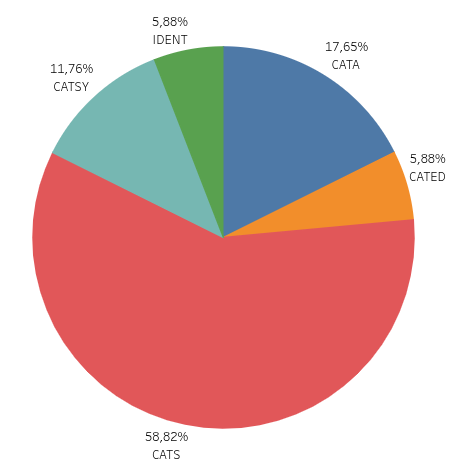
\includegraphics[width=0.5\linewidth]{./illustrations/graph_FR2_2.png}
	\caption{Visualisation par secteur du \gls{td} de la collection \enquote{13h15 l'après-midi}}
	\label{fig:traitement_secteur}
\end{figure}

En cliquant sur un résultat, une fiche s'affiche dispensant certaines informations sur la chaîne ou l'émission permettant de les situer dans le temps. Tout cela accompagné bien des graphiques en barre, représentés dans le \hyperref[fig:traitement_FR2]{chapitre précédent}. Ces graphiques sont personnalisables selon l'information que l'utilisateur recherche, en définissant des dates extrêmes pour les deux typologies (chaîne et émission) et en ajoutant des filtres pour choisir le genre pour la fiche chaîne. Auquel se rajoute le graphique de \gls{td} des genres sur cette chaîne. Avec cette structure, les utilisateurs suivent un cheminement simple, il y a peu de pages, toutes visibles dès la page d'accueil avec une organisation comportant strictement les informations dont les utilisateurs ont besoin pour construire le corpus dont ils ont besoin : identification du document ou de la collection et traitement appliqué, selon leurs critères personnalisés. 

\subsection{Garantir la lisibilité des informations : les datavisualisations}

Pour correspondre à l'expérience que nous souhaitons offrir, la notion de \gls{td} ne doit pas repousser l'utilisateur. C'est pourquoi nous avons fait appel aux datavisualisations. La représentation graphique simplifie visuellement l'information et en gardant le même code couleur pour chaque type de traitement sur l'ensemble de l'outil, les informations concernant le \gls{td} est plus facilement intégrable et l'ensemble des résultats et notices répondant aux mêmes codes visuels, l'utilisateur peut mobiliser rapidement l'information. 

%% Conclusion %%

Une des manières dont nous avons choisi de concrétiser cette expérience utilisateur favorable est l'utilisation des filtres afin de permettre à l'utilisateur de personnaliser au maximum sa recherche. 